\documentclass{beamer}

\usepackage{amsmath,amssymb,booktabs,tabularx,array}
\usetheme{sintef}
\usepackage{xeCJK}
\usepackage{tikz}
\usetikzlibrary{arrows.meta,positioning,calc}

\setCJKmainfont[AutoFakeBold=2.5]{WenQuanYi Zen Hei}
\setCJKsansfont[AutoFakeBold=2.5]{WenQuanYi Zen Hei}
\usefonttheme[onlymath]{serif}

\titlebackground*{assets/background}
\title{透明物体 Baseline 复现进度}
\subtitle{Baseline $\rightarrow$ DepthHypothesisPack v1 $\rightarrow$ 下一阶段 gate}
\author{MDE Research}
\date{2026.09.01}

\definecolor{ink}{RGB}{42,45,52}
\definecolor{accentblue}{RGB}{40,103,178}
\definecolor{accentorange}{RGB}{230,118,40}
\definecolor{good}{RGB}{30,142,92}
\definecolor{warn}{RGB}{201,132,34}
\definecolor{bad}{RGB}{190,60,55}
\definecolor{softblue}{RGB}{235,243,252}
\definecolor{softorange}{RGB}{253,243,234}
\definecolor{softgreen}{RGB}{234,248,241}
\definecolor{softgrey}{RGB}{244,244,242}

\setbeamercolor{normal text}{fg=ink,bg=white}
\setbeamercolor{cardblue}{fg=ink,bg=softblue}
\setbeamercolor{cardorange}{fg=ink,bg=softorange}
\setbeamercolor{cardgreen}{fg=ink,bg=softgreen}
\setbeamercolor{cardgrey}{fg=ink,bg=softgrey}
\setbeamercolor{keybox}{fg=white,bg=maincolor}
\setbeamersize{text margin left=0.75cm,text margin right=0.75cm}
\setlength{\tabcolsep}{4pt}

% Keep the template's section subtitle, but suppress automatic TOC slides.
\AtBeginSection[]{}

\newcommand{\ok}{\textcolor{good}{\ensuremath{\checkmark}}}
\newcommand{\caution}{\textcolor{warn}{\ensuremath{\triangle}}}
\newcommand{\source}[1]{%
  \par\vspace{0.25em}{\color{gray}\fontsize{5.8}{6.6}\selectfont 数据源：#1}\par
}
\newcommand{\cardtitle}[1]{\textcolor{maincolor}{\bfseries #1}}
\newcommand{\pill}[2]{%
  \tikz[baseline=(p.base)]\node[rounded corners=2pt,fill=#1,inner xsep=5pt,inner ysep=2pt]
  (p){\fontsize{6.3}{7}\selectfont\bfseries #2};%
}

\begin{document}

\maketitle

\section{全景}

\begin{frame}{路线图：先把比较尺子做对，再验证 Idea}
\vspace{-0.35em}
\begin{columns}[T,onlytextwidth]
  \begin{column}{0.318\textwidth}
    \begin{beamercolorbox}[wd=\linewidth,sep=0.85em,rounded=true]{cardblue}
      \cardtitle{原生 benchmark}

      \vspace{0.45em}\small
      \ok\ Depth4ToM Base / Booster

      \ok\ DFNet / TransCG full

      \ok\ ReMake / TransCG full

      \vspace{0.6em}\scriptsize
      论文或官方协议下的模型分数
    \end{beamercolorbox}
  \end{column}
  \begin{column}{0.318\textwidth}
    \begin{beamercolorbox}[wd=\linewidth,sep=0.85em,rounded=true]{cardorange}
      \cardtitle{多层主基线}

      \vspace{0.45em}\small
      \ok\ LayeredDepth val（300）

      \ok\ SeeGroup val / teacher 审计

      \ok\ 双向 bridge diagnostics

      \vspace{0.6em}\scriptsize
      单层与多层放进同一评测
    \end{beamercolorbox}
  \end{column}
  \begin{column}{0.318\textwidth}
    \begin{beamercolorbox}[wd=\linewidth,sep=0.85em,rounded=true]{cardgreen}
      \cardtitle{我们的模型与下游}

      \vspace{0.45em}\small
      \ok\ DHP ResNet / DINOv2-S

      \ok\ 尺度锚定诊断

      \ok\ ShellBench / frozen planner

      \vspace{0.6em}\scriptsize
      同一协议定位真实失败模式
    \end{beamercolorbox}
  \end{column}
\end{columns}

\vspace{0.7em}
\begin{beamercolorbox}[wd=\linewidth,sep=0.65em,rounded=true]{cardgrey}
\centering\small
\pill{softblue}{原生复现} 官方数据 / checkpoint / evaluator
\quad
\pill{softorange}{统一 benchmark} 我们的共同协议
\quad
\pill{softgreen}{诊断 / oracle} 隔离表示上限
\end{beamercolorbox}

\vspace{0.55em}
\centering
\textcolor{maincolor}{\bfseries 当前结论：多层表示信号成立，但 DHP 主性能 gate 未通过；下一步应解决域对齐。}
\source{baseline\_results\_2026-08-30.json；depth\_hypothesis\_pack\_v1\_results\_2026-08-31.json。}
\end{frame}

\section{原生 benchmark}

\begin{frame}{Step 1｜比较尺子可信吗？原生结果已对齐}
\vspace{-0.5em}
\begin{columns}[T,onlytextwidth]
  \begin{column}{0.47\textwidth}
    \cardtitle{Depth4ToM code path · Booster（228）}

    \vspace{0.35em}
    \renewcommand{\arraystretch}{1.35}
    \scriptsize
    \begin{tabularx}{\linewidth}{@{}Xrrc@{}}
      \toprule
      Model & 本地 ToM RMSE & 论文 & 状态 \\
      \midrule
      MiDaS v2.1 Base & 140.40 mm & 140.31 & \ok \\
      DPT-Large Base  & 136.28 mm & 136.28 & \ok \\
      \bottomrule
    \end{tabularx}

    \vspace{0.7em}
    \begin{beamercolorbox}[wd=\linewidth,sep=0.65em,rounded=true]{cardorange}
      \scriptsize
      \textbf{边界：}这里只能称为 \textbf{Base}。Depth4ToM FT checkpoint 未公开，不能宣称已复现 FT。
    \end{beamercolorbox}
  \end{column}
  \begin{column}{0.49\textwidth}
    \cardtitle{TransCG official test（52 scenes / 23,524）}

    \vspace{0.35em}
    \renewcommand{\arraystretch}{1.24}
    \scriptsize
    \begin{tabularx}{\linewidth}{@{}Xrr@{}}
      \toprule
      Masked metric & 本地 ReMake & 论文 Table I \\
      \midrule
      RMSE $\downarrow$ & 0.010854 m & 0.011 m \\
      REL $\downarrow$  & 0.016906 & 0.017 \\
      MAE $\downarrow$  & 0.007532 m & 0.008 m \\
      $\delta_{1.05}$ $\uparrow$ & 93.9086\% & 93.91\% \\
      \bottomrule
    \end{tabularx}

    \vspace{0.55em}
    \scriptsize
    \ok\ \textbf{ReMake：}全部 masked 指标在论文报告精度内一致。

    \vspace{0.2em}
    \caution\ \textbf{DFNet current release：}masked RMSE 0.032787 m；全量完成，但 checkpoint 与论文旧版不同。
  \end{column}
\end{columns}

\vspace{0.75em}
\begin{beamercolorbox}[wd=\linewidth,sep=0.52em,rounded=true]{cardgreen}
\centering\small
TransCG 数据已完整下载并审计：\textbf{13 个分卷、23,524 个样本、CRC / 结构检查通过}。
\end{beamercolorbox}
\source{Depth4ToM official evaluator；TransCG native evaluators；ReMake Global Loss。}
\end{frame}

\section{核心 gap}

\begin{frame}{Step 2｜为什么需要多层？single-depth 丢失界面}
\vspace{-0.55em}
\begin{columns}[T,onlytextwidth]
  \begin{column}{0.37\textwidth}
    \centering
    \includegraphics[width=\linewidth]{../assets/seegroup_core.png}

    \vspace{0.25em}
    \fontsize{6}{7}\selectfont
    一条相机射线可穿过多个介质界面；只保留最近表面，会直接丢掉内壁与后壁。
  \end{column}
  \begin{column}{0.60\textwidth}
    \centering
    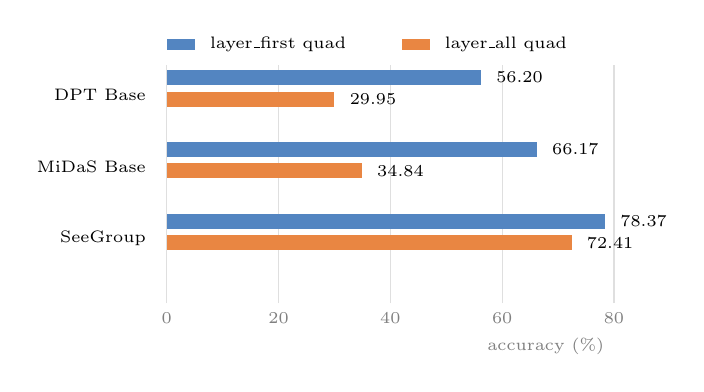
\begin{tikzpicture}[x=0.071cm,y=0.48cm,font=\fontsize{6.5}{7.2}\selectfont]
      \foreach \x in {0,20,40,60,80} {
        \draw[gray!25] (\x,-0.15) -- (\x,6.15);
        \node[gray,anchor=north] at (\x,-0.15) {\x};
      }
      \node[anchor=east] at (-2,5.35) {DPT Base};
      \node[anchor=east] at (-2,3.45) {MiDaS Base};
      \node[anchor=east] at (-2,1.55) {SeeGroup};

      \fill[accentblue!80] (0,5.62) rectangle (56.198,6.02);
      \fill[accentorange!88] (0,5.05) rectangle (29.954,5.45);
      \fill[accentblue!80] (0,3.72) rectangle (66.166,4.12);
      \fill[accentorange!88] (0,3.15) rectangle (34.842,3.55);
      \fill[accentblue!80] (0,1.82) rectangle (78.372,2.22);
      \fill[accentorange!88] (0,1.25) rectangle (72.414,1.65);

      \node[anchor=west] at (57.2,5.82) {56.20};
      \node[anchor=west] at (31.0,5.25) {29.95};
      \node[anchor=west] at (67.2,3.92) {66.17};
      \node[anchor=west] at (35.9,3.35) {34.84};
      \node[anchor=west] at (79.4,2.02) {78.37};
      \node[anchor=west] at (73.4,1.45) {72.41};

      \fill[accentblue!80] (0,6.55) rectangle (5,6.85);
      \node[anchor=west] at (6,6.7) {layer\_first quad};
      \fill[accentorange!88] (42,6.55) rectangle (47,6.85);
      \node[anchor=west] at (48,6.7) {layer\_all quad};
      \node[gray,anchor=north east] at (80,-0.82) {accuracy (\%)};
    \end{tikzpicture}
  \end{column}
\end{columns}

\vspace{0.45em}
\begin{columns}[T,onlytextwidth]
  \begin{column}{0.49\textwidth}
    \begin{beamercolorbox}[wd=\linewidth,sep=0.55em,rounded=true]{keybox}
      \centering
      \Large\bfseries +37.572 pp

      \scriptsize SeeGroup vs 最强 single-depth 的 layer\_all gap
    \end{beamercolorbox}
  \end{column}
  \begin{column}{0.49\textwidth}
    \begin{beamercolorbox}[wd=\linewidth,sep=0.55em,rounded=true]{cardorange}
      \centering
      \large\bfseries mixed-layer：0\% vs 66.610\%

      \scriptsize DPT / MiDaS 无法回答跨层 quadruplet
    \end{beamercolorbox}
  \end{column}
\end{columns}
\source{LayeredDepth validation，300 images；195,800 mixed-layer quadruplets。}
\end{frame}

\begin{frame}{Step 3｜能直接拼接吗？multi-layer 尚未米制对齐}
\vspace{-0.2em}
\centering
\small SeeGroup closest layer $\rightarrow$ Booster ToM（228）

\vspace{0.55em}
\begin{columns}[T,onlytextwidth]
  \begin{column}{0.455\textwidth}
    \begin{beamercolorbox}[wd=\linewidth,sep=1.0em,rounded=true]{cardorange}
      \centering
      \scriptsize 直接把 raw head 当米制

      \vspace{0.25em}
      {\fontsize{22}{24}\selectfont\bfseries\textcolor{bad}{3372.31}}

      \small mm ToM RMSE

      \vspace{0.4em}\scriptsize AbsRel 3.7827 · $\delta_{1.05}$ 0.00018\%
    \end{beamercolorbox}
  \end{column}
  \begin{column}{0.07\textwidth}
    \centering\vspace{2.25em}
    \textcolor{maincolor}{\Large$\Rightarrow$}
  \end{column}
  \begin{column}{0.455\textwidth}
    \begin{beamercolorbox}[wd=\linewidth,sep=1.0em,rounded=true]{cardgreen}
      \centering
      \scriptsize Depth4ToM affine alignment 后

      \vspace{0.25em}
      {\fontsize{22}{24}\selectfont\bfseries\textcolor{good}{65.54}}

      \small mm ToM RMSE

      \vspace{0.4em}\scriptsize AbsRel 0.0642 · $\delta_{1.05}$ 44.24\%
    \end{beamercolorbox}
  \end{column}
\end{columns}

\vspace{0.75em}
\begin{tikzpicture}[node distance=0.7cm,>=Latex,font=\small]
  \node[draw=accentblue,fill=softblue,rounded corners,minimum width=4.0cm,minimum height=0.95cm]
    (multi) {多层相对结构};
  \node[draw=maincolor,fill=maincolor!8,rounded corners,minimum width=4.5cm,minimum height=0.95cm,right=of multi]
    (bridge) {域对齐 + 多界面监督};
  \node[draw=good,fill=softgreen,rounded corners,minimum width=4.0cm,minimum height=0.95cm,right=of bridge]
    (metric) {米制 single-depth readout};
  \draw[->,very thick,accentblue] (multi) -- (bridge);
  \draw[->,very thick,good] (bridge) -- (metric);
\end{tikzpicture}

\vspace{0.55em}
\textcolor{maincolor}{\bfseries 51.46$\times$ 的差异说明：结构信息是可用的，但输出空间没有对齐。}

\vspace{0.2em}\scriptsize
这不是 SeeGroup 的原生失败分数，而是跨协议 calibration stress test。
\source{SeeGroup released checkpoint；Booster ToM protocol。}
\end{frame}

\section{DepthHypothesisPack}

\begin{frame}{Step 4｜我们的尝试：固定多层 Head，受控筛选 encoder}
\vspace{-0.5em}
\begin{beamercolorbox}[wd=\linewidth,sep=0.45em,rounded=true]{cardgrey}
\centering\small
RGB $\rightarrow$ encoder $\rightarrow$
$d_1 < d_2 < d_3 < d_4$ + monotone presence + uncertainty

\scriptsize 同一 K=4 head、loss、synthetic split、校准与 evaluator
\end{beamercolorbox}

\vspace{0.55em}
\begin{columns}[T,onlytextwidth]
  \begin{column}{0.43\textwidth}
    \cardtitle{1k frozen pilot：谁值得扩大？}

    \vspace{0.35em}
    \renewcommand{\arraystretch}{1.28}
    \scriptsize
    \begin{tabularx}{\linewidth}{@{}Xrrr@{}}
      \toprule
      Encoder & Depth MAE $\downarrow$ & Front $\downarrow$ & Pres. F1 $\uparrow$ \\
      \midrule
      \textbf{DINOv2-S} & \textbf{0.522} & \textbf{0.465} & \textbf{0.9005} \\
      Depth Anything V2-S & 0.537 & 0.477 & 0.8755 \\
      \bottomrule
    \end{tabularx}

    \vspace{0.55em}
    \scriptsize
    \ok\ DINO 扩大到 14,800 张；\quad
    \caution\ DA-V2 按 pilot gate 停止。
  \end{column}
  \begin{column}{0.54\textwidth}
    \cardtitle{真实 LayeredDepth：结构是否增强？}

    \vspace{0.35em}
    \renewcommand{\arraystretch}{1.22}
    \scriptsize
    \begin{tabularx}{\linewidth}{@{}Xrrr@{}}
      \toprule
      Method & First & All & Mixed \\
      \midrule
      MiDaS Base & 66.17 & 34.84 & 0.00 \\
      DHP ResNet & 41.63 & 32.04 & 20.45 \\
      \textbf{DHP DINOv2-S} & 39.59 & \textbf{32.91} & \textbf{25.12} \\
      SeeGroup & \textbf{78.37} & \textbf{72.41} & \textbf{66.61} \\
      \bottomrule
    \end{tabularx}
  \end{column}
\end{columns}

\vspace{0.4em}
\begin{beamercolorbox}[wd=\linewidth,sep=0.55em,rounded=true]{keybox}
\centering
\large\bfseries Mixed quad：20.45\% $\rightarrow$ 25.12\% \quad 但 \quad TablewareNet interface F1：0.422\%

\scriptsize 更强 encoder 提升跨层排序，却没有解决 synthetic $\rightarrow$ operation domain 的米制迁移
\end{beamercolorbox}
\source{LayeredDepth-Syn train only；ResNet formal fine-tuned，DINO / DA frozen；真实数据均为 evaluation-only。}
\end{frame}

\section{统一 ShellBench}

\begin{frame}{Step 5｜失败在哪里？主要是域与米制界面对齐}
\vspace{-0.5em}
\begin{beamercolorbox}[wd=\linewidth,sep=0.45em,rounded=true]{cardgrey}
\centering\scriptsize
100 scenes / 700 RGB views · 98 hollow-scored scenes · 259 objects · 1,813 event maps · 139.2M rays
\end{beamercolorbox}

\vspace{0.45em}
\renewcommand{\arraystretch}{1.18}
\scriptsize
\begin{tabularx}{\linewidth}{@{}Xlrr@{}}
  \toprule
  Readout & 性质 & Interface F1 $\uparrow$ & Transition F1 $\uparrow$ \\
  \midrule
  T²SQNet + GT mask & multi-layer oracle input & \textbf{79.23\%} & \textbf{73.59\%} \\
  T²SQNet + RGB / LangSAM & multi-layer end-to-end & 74.27\% & 69.14\% \\
  Perfect rendered front & single-depth upper bound & 43.104\% & --- \\
  DHP ResNet formal & synthetic $\rightarrow$ OOD & 0.924\% & --- \\
  \textbf{DHP DINOv2-S} & synthetic $\rightarrow$ OOD & 0.422\% & --- \\
  DHP DINO + bg affine$^*$ & scale oracle diagnostic & \textbf{1.693\%} & --- \\
  \bottomrule
\end{tabularx}

\vspace{0.55em}
\begin{columns}[T,onlytextwidth]
  \begin{column}{0.49\textwidth}
    \begin{beamercolorbox}[wd=\linewidth,sep=0.58em,rounded=true]{cardorange}
      \centering
      \large\bfseries 不是一个全局 scale

      \scriptsize 即使用 test GT 求最优 affine，front MAE 仍有 88 mm
    \end{beamercolorbox}
  \end{column}
  \begin{column}{0.49\textwidth}
    \begin{beamercolorbox}[wd=\linewidth,sep=0.58em,rounded=true]{cardblue}
      \centering
      \large\bfseries 尺度修正有用，但远远不够

      \scriptsize bg affine：0.422\% $\rightarrow$ 1.693\%，仍远低于 43.104\%
    \end{beamercolorbox}
  \end{column}
\end{columns}

\vspace{0.4em}\centering\small
\textcolor{maincolor}{\bfseries 结论：瓶颈是域内米制 / interface 监督，而不是继续堆通用 encoder。}

\source{DHP 使用 GT identity / association / rendered-front visibility adapter；$^*$另用 test bg depth + GT union mask。}
\end{frame}

\begin{frame}{Step 6｜多层预测改善动作了吗？还没有过 gate}
\vspace{-0.45em}
\begin{beamercolorbox}[wd=\linewidth,sep=0.45em,rounded=true]{cardgrey}
\centering\scriptsize
同一批 \textbf{244 matched objects / 7,983 frozen candidates}；数字均为 safe / collision / reject
\end{beamercolorbox}

\vspace{0.5em}
\renewcommand{\arraystretch}{1.3}
\scriptsize
\begin{tabularx}{\linewidth}{@{}Xccc@{}}
  \toprule
  输入几何 & Front optimistic & Front conservative & K-event parity \\
  \midrule
  DHP ResNet formal & 223 / 21 / 0 & 197 / 5 / 42 & 198 / 5 / 41 \\
  \textbf{DHP DINO raw} & 226 / 18 / 0 & 228 / 5 / 11 & \textbf{229 / 5 / 10} \\
  DINO + bg affine$^*$ & 227 / 16 / 1 & 206 / 2 / 36 & 211 / 2 / 31 \\
  \midrule
  GT shell oracle & 224 / 20 / 0 & 240 / 0 / 4 & \textbf{244 / 0 / 0} \\
  \bottomrule
\end{tabularx}

\vspace{0.65em}
\begin{columns}[T,onlytextwidth]
  \begin{column}{0.49\textwidth}
    \begin{beamercolorbox}[wd=\linewidth,sep=0.62em,rounded=true]{cardgreen}
      \centering
      \large\bfseries 表示上限成立

      \scriptsize GT full events：244 safe / 0 collision / 0 reject
    \end{beamercolorbox}
  \end{column}
  \begin{column}{0.49\textwidth}
    \begin{beamercolorbox}[wd=\linewidth,sep=0.62em,rounded=true]{cardorange}
      \centering
      \large\bfseries 当前模型质量不足

      \scriptsize affine 将 collision 5 $\rightarrow$ 2，却使 safe 229 $\rightarrow$ 211
    \end{beamercolorbox}
  \end{column}
\end{columns}

\vspace{0.55em}
\centering\small
\textcolor{maincolor}{\bfseries 所以现在训练 planner head，只会让下游学习上游的几何错误。}

\source{$^*$尺度 oracle；offline target-shell collision gate，不是机器人 task success。}
\end{frame}

\section{结论}

\begin{frame}{Decision｜不再堆 baseline / encoder，转向域对齐训练}
\vspace{-0.45em}
\begin{beamercolorbox}[wd=\linewidth,sep=0.75em,rounded=true]{keybox}
\centering
\large\bfseries Idea 有表示层证据；当前失败点已定位为 synthetic $\rightarrow$ operation domain 对齐。
\end{beamercolorbox}

\vspace{0.4em}
\begin{columns}[T,onlytextwidth]
  \begin{column}{0.44\textwidth}
    \cardtitle{我们现在确定知道什么}

    \vspace{0.35em}\small
    \ok\ Baseline 与统一 benchmark 已冻结

    \ok\ K=4 mixed signal：20.45\% $\rightarrow$ 25.12\%

    \caution\ DINO direct interface F1 仅 0.422\%

    \caution\ Scale oracle 也只有 1.693\%

    \ok\ SeeGroup raw teacher / 简单 scale 已审计

    \ok\ 46 unit + 2 integration checks 全通过

    \vspace{0.55em}
    \begin{beamercolorbox}[wd=\linewidth,sep=0.5em,rounded=true]{cardorange}
      \centering\scriptsize
      \textbf{暂不做：}更多重型复现、扩大 test benchmark、transition / learned planner
    \end{beamercolorbox}
  \end{column}
  \begin{column}{0.53\textwidth}
    \cardtitle{下一项唯一有信息量的实验}

    \vspace{0.45em}
    \begin{tikzpicture}[node distance=0.35cm,font=\scriptsize,>=Latex]
      \node[draw=accentblue,fill=softblue,rounded corners,text width=7.5cm,minimum height=0.72cm,align=left]
        (a) {\textbf{1}\quad TablewareNet training 3,000 scenes：导出 physical-shell GT};
      \node[draw=maincolor,fill=maincolor!7,rounded corners,text width=7.5cm,minimum height=0.72cm,align=left,below=of a]
        (b) {\textbf{2}\quad 小 pilot：synthetic ordering + 域内 metric / interface};
      \node[draw=accentorange,fill=softorange,rounded corners,text width=7.5cm,minimum height=0.72cm,align=left,below=of b]
        (c) {\textbf{3}\quad 独立 validation 100 scenes：选模型 / 校准 / 过 gate};
      \node[draw=good,fill=softgreen,rounded corners,text width=7.5cm,minimum height=0.72cm,align=left,below=of c]
        (d) {\textbf{4}\quad 配置冻结后，只跑一次现有 test 100 scenes};
      \node[draw=gray,fill=softgrey,rounded corners,text width=7.5cm,minimum height=0.72cm,align=left,below=of d]
        (e) {\textbf{5}\quad 过 gate 后，再加 transition / planner head};
      \draw[->,gray!70] (a) -- (b);
      \draw[->,gray!70] (b) -- (c);
      \draw[->,gray!70] (c) -- (d);
      \draw[->,gray!70] (d) -- (e);
    \end{tikzpicture}
  \end{column}
\end{columns}

\vspace{0.25em}
\centering\scriptsize
主表继续分开：\textbf{TransCG metric depth}｜\textbf{LayeredDepth multi-layer}｜\textbf{ShellBench interfaces / collision}；现有 test 保持冻结。
\source{DepthHypothesisPack v1 强编码器与尺度诊断（2026-08-31）。}
\end{frame}

\end{document}
